\documentclass[12pt,a4paper]{article}
\usepackage[utf8]{vietnam}
\usepackage{amsmath}
\usepackage{amsfonts}
\usepackage{amssymb}
\usepackage{caption}
\usepackage{subcaption}
\usepackage{graphicx}
\title{Introduction to Smart Trash}
\author{Group 1 - BB LAB}
\date{January 2023}
\begin{document}
\maketitle
\begin{abstract}
  Ở bản báo cáo này, chúng ta sẽ đặt vấn đề, tìm hiểu về thùng rác thông minh, tìm hiểu và lựa chọn thiết bị đấu nối, kết luận sản phẩm.
\end{abstract}
\tableofcontents
\newpage
\section{Đặt Vấn Đề}
\subsection{Lý Do Chọn Đề Tài} 
Rác thải đang là một thực trạng đáng báo động trên toàn cầu. Mỗi một ngày lượng rác thải ra ngoài môi trường là vô cùng nhiều. Đồng thời khoa học kĩ thuật trên đà phát triển rất mạnh, nhiều ngành nghề đã được áp dụng khoa học kĩ thuật vào, kể những đồ dùng đơn giản trong gia đình cũng có rất nhiều đồ dùng thông minh và đòi hỏi kĩ thuật. Vậy nên tôi đã lựa chọn một đề tài nhỏ là
chiếc "Thùng Rác Thông Minh".
\subsection{Mục Tiêu Kỹ Thuật}
\begin{enumerate}
    \item Sản phẩm an toàn với mọi người.
    \item Sản phẩm lắp ráp đơn giản và gọn nhẹ.
    \item Sản phẩm thiết kế đơn giản tận dụng ngay được thùng rác bình thường trong nhà.
\end{enumerate}
\section{Tìm Hiểu Chung Về Thùng Rác Thông Minh}
\subsection{Thùng Rác Thông Minh Là Gì?}
\hspace{0.7cm}Ngày nay, với sự phát triển nhanh chóng của công nghệ và khoa học kĩ thuật, những nhà nghiên cứu đã không ngừng đưa ra những phát minh mới mang tính ứng dụng trong cuộc sống thường ngày, thùng rác thông minh là một sản phẩm như vậy. Thùng rác thông minh ứng dụng công nghệ cảm ứng siêu âm để giúp đóng mở dễ dàng hơn.
\newpage
\begin{figure}
    \centering
    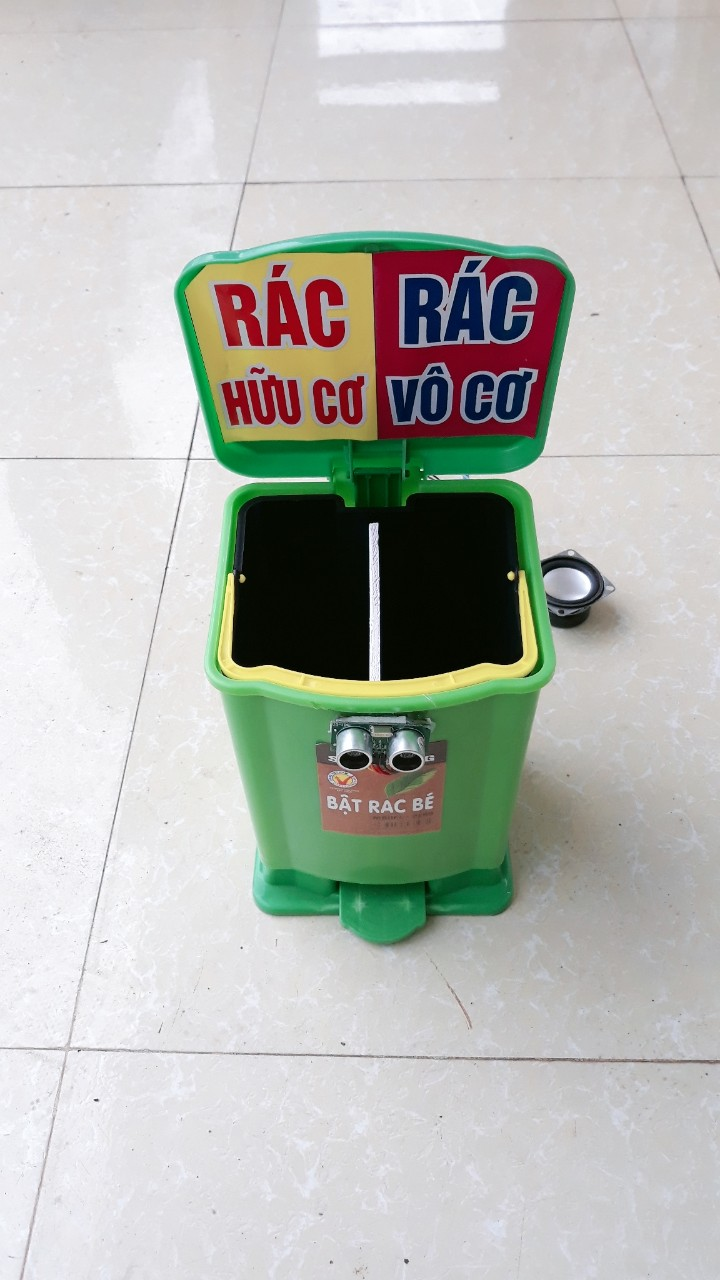
\includegraphics[scale=0.2]{hinh 1}
    \caption{\textit{Thùng rác thông minh tự chế :))}}
    \label{fig1}
\end{figure}
\subsection{Nó Có Gì Khác So Với Thùng Rác Bình Thường}
\hspace{0.7cm}Khác với các loại thùng rác thông thường bạn phải dùng tay hoặc chân để có thể sử dụng, thì đối với thùng rác thông minh nó có chức năng tự động mở lắp thùng khi gặp vật cản khoảng 15-20 cm, và đóng lại sau 3-5 giây. Người dùng chỉ cần đưa tay vào vùng cảm ứng, thùng rác sẽ mở ra tự động nhờ có các chip máy tính, và các thiết bị được trang bị trên thùng rác.
\subsection{Những Đặc Điểm Nổi Bật Của Thùng Rác Thông Minh}
\begin{itemize}
    \item \textbf{Tính năng hiện đại}: Với tính năng cảm biến khoảng cách, thùng rác thông minh cho phép người sử dụng vứt rác mà không cần dùng tay hoặc chân để đóng mở lắp.
    \item \textbf{Đảm bảo vệ sinh}: Không cần phải chạm tay vào thùng rác có thể tránh được lây lan của vi khuẩn.
    \item \textbf{Góp phần nâng cao ý thức giữ gìn vệ sinh}: Có một số người bị "bệnh lười vứt rác" do không muốn dùng tay chân/ tay để mở lắp thùng rác. Nhưng thùng rác thông minh có thể trị được bệnh lười này.
\end{itemize} 
\section{Tìm Hiểu, Lựa Chọn Thiết Bị Và Đầu Nối}
\subsection{Lựa Chọn Thiết Bị}
\begin{itemize}
    \item Mạch Arduino Uno R3\\
    \textbf{Thông số kỹ thuật:}
\end{itemize}
$-$ Thiết kế theo đúng chuẩn chân, kích thước của Arduino Uno chính hãng.\\
$-$ IC chính: ATmega328P-AU.\\
$-$ IC nạp và giao tiếp UART: CH340.\\
$-$ Điện áp cấp: 5VDC cổng USB, 6-9VDC chân Raw.\\
$-$ Mức điện áp giao tiếp GPIO: TTL 5VDC.\\
$-$ Dòng GPIO: 30mA.\\
$-$ Số chân Digital: 14 chân, trong đó có 6 chân PWM.\\
$-$ Số chân Analog: 6 chân.\\
$-$ Flash Memory: 32KB (2KB Bootloader).\\
$-$ SRAM: 2KB.\\
$-$ EEPROM: 1KB.\\
$-$ Clock Speed: 16Mhz.\\
$-$ Tích hợp Led báo nguồn, led chân D13, LED RX, TX.\\
$-$ Tích hợp IC chuyển điện áp 5V LM1117.\\
$-$ Khối lượng: 25g.
\begin{figure}[ht!]
    \centering
    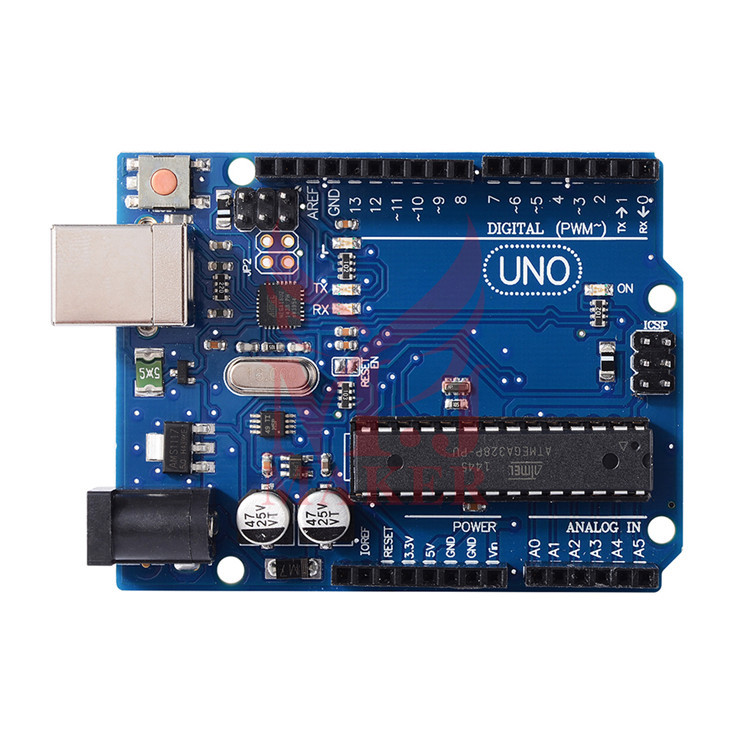
\includegraphics[scale=0.3]{hinh 2.jpg}
    \caption{\textit{Arduino Uno R3.}}
    \label{fig2}
\end{figure}
\newpage
\begin{itemize}
    \item Cảm Biến Siêu Âm\\
    \textbf{Thông số kỹ thuật của cảm biến siêu âm HC-SR04:}
\end{itemize}
$-$ Điện áp: 5VDC.\\
$-$ Dòng hoạt động: <2mA.\\
$-$ Mức cao: 5V.\\
$-$ Mức thấp: 0V.\\
$-$ Góc tối đa: 15 độ.\\
$-$ Khoảng cách: 2cm - 450cm (4.5m).\\
$-$ Độ chính xác: 3mm.
\begin{figure}[ht!]
    \centering
    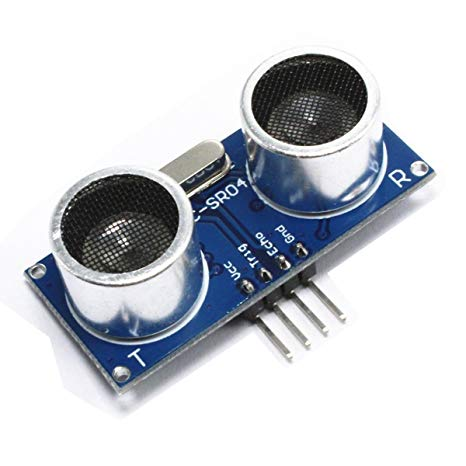
\includegraphics[scale=0.5]{hinh 3.jpg}
    \caption{\textit{Cảm biến siêu âm.}}
    \label{fig3}
\end{figure}
\newpage
\begin{itemize}
    \item Động Cơ Servo\\
    \textbf{Thông số kỹ thuật của động cơ Servo SG90}
\end{itemize}
$-$ Động cơ servo SG90 có thể quay 180 độ.\\
$-$ Kích thước: 22.2 x 11.8 x 32 mm.\\
$-$ Điện áp hoạt động: 4.8V (~5V).\\
$-$ Động cơ servo có thể đạt góc quay chính xác trong khoảng 90 - 180 độ.\\
$-$ Khối lượng : 9g.\\
$-$ Momen xoắn: 1.8kg/cm\\
$-$ Tốc độ hoạt động: 60 độ trong 0.1 giây.\\
$-$ Nhiệt độ hoạt động: 0 ℃ - 55 ℃.\\
\begin{figure}[ht!]
    \centering
    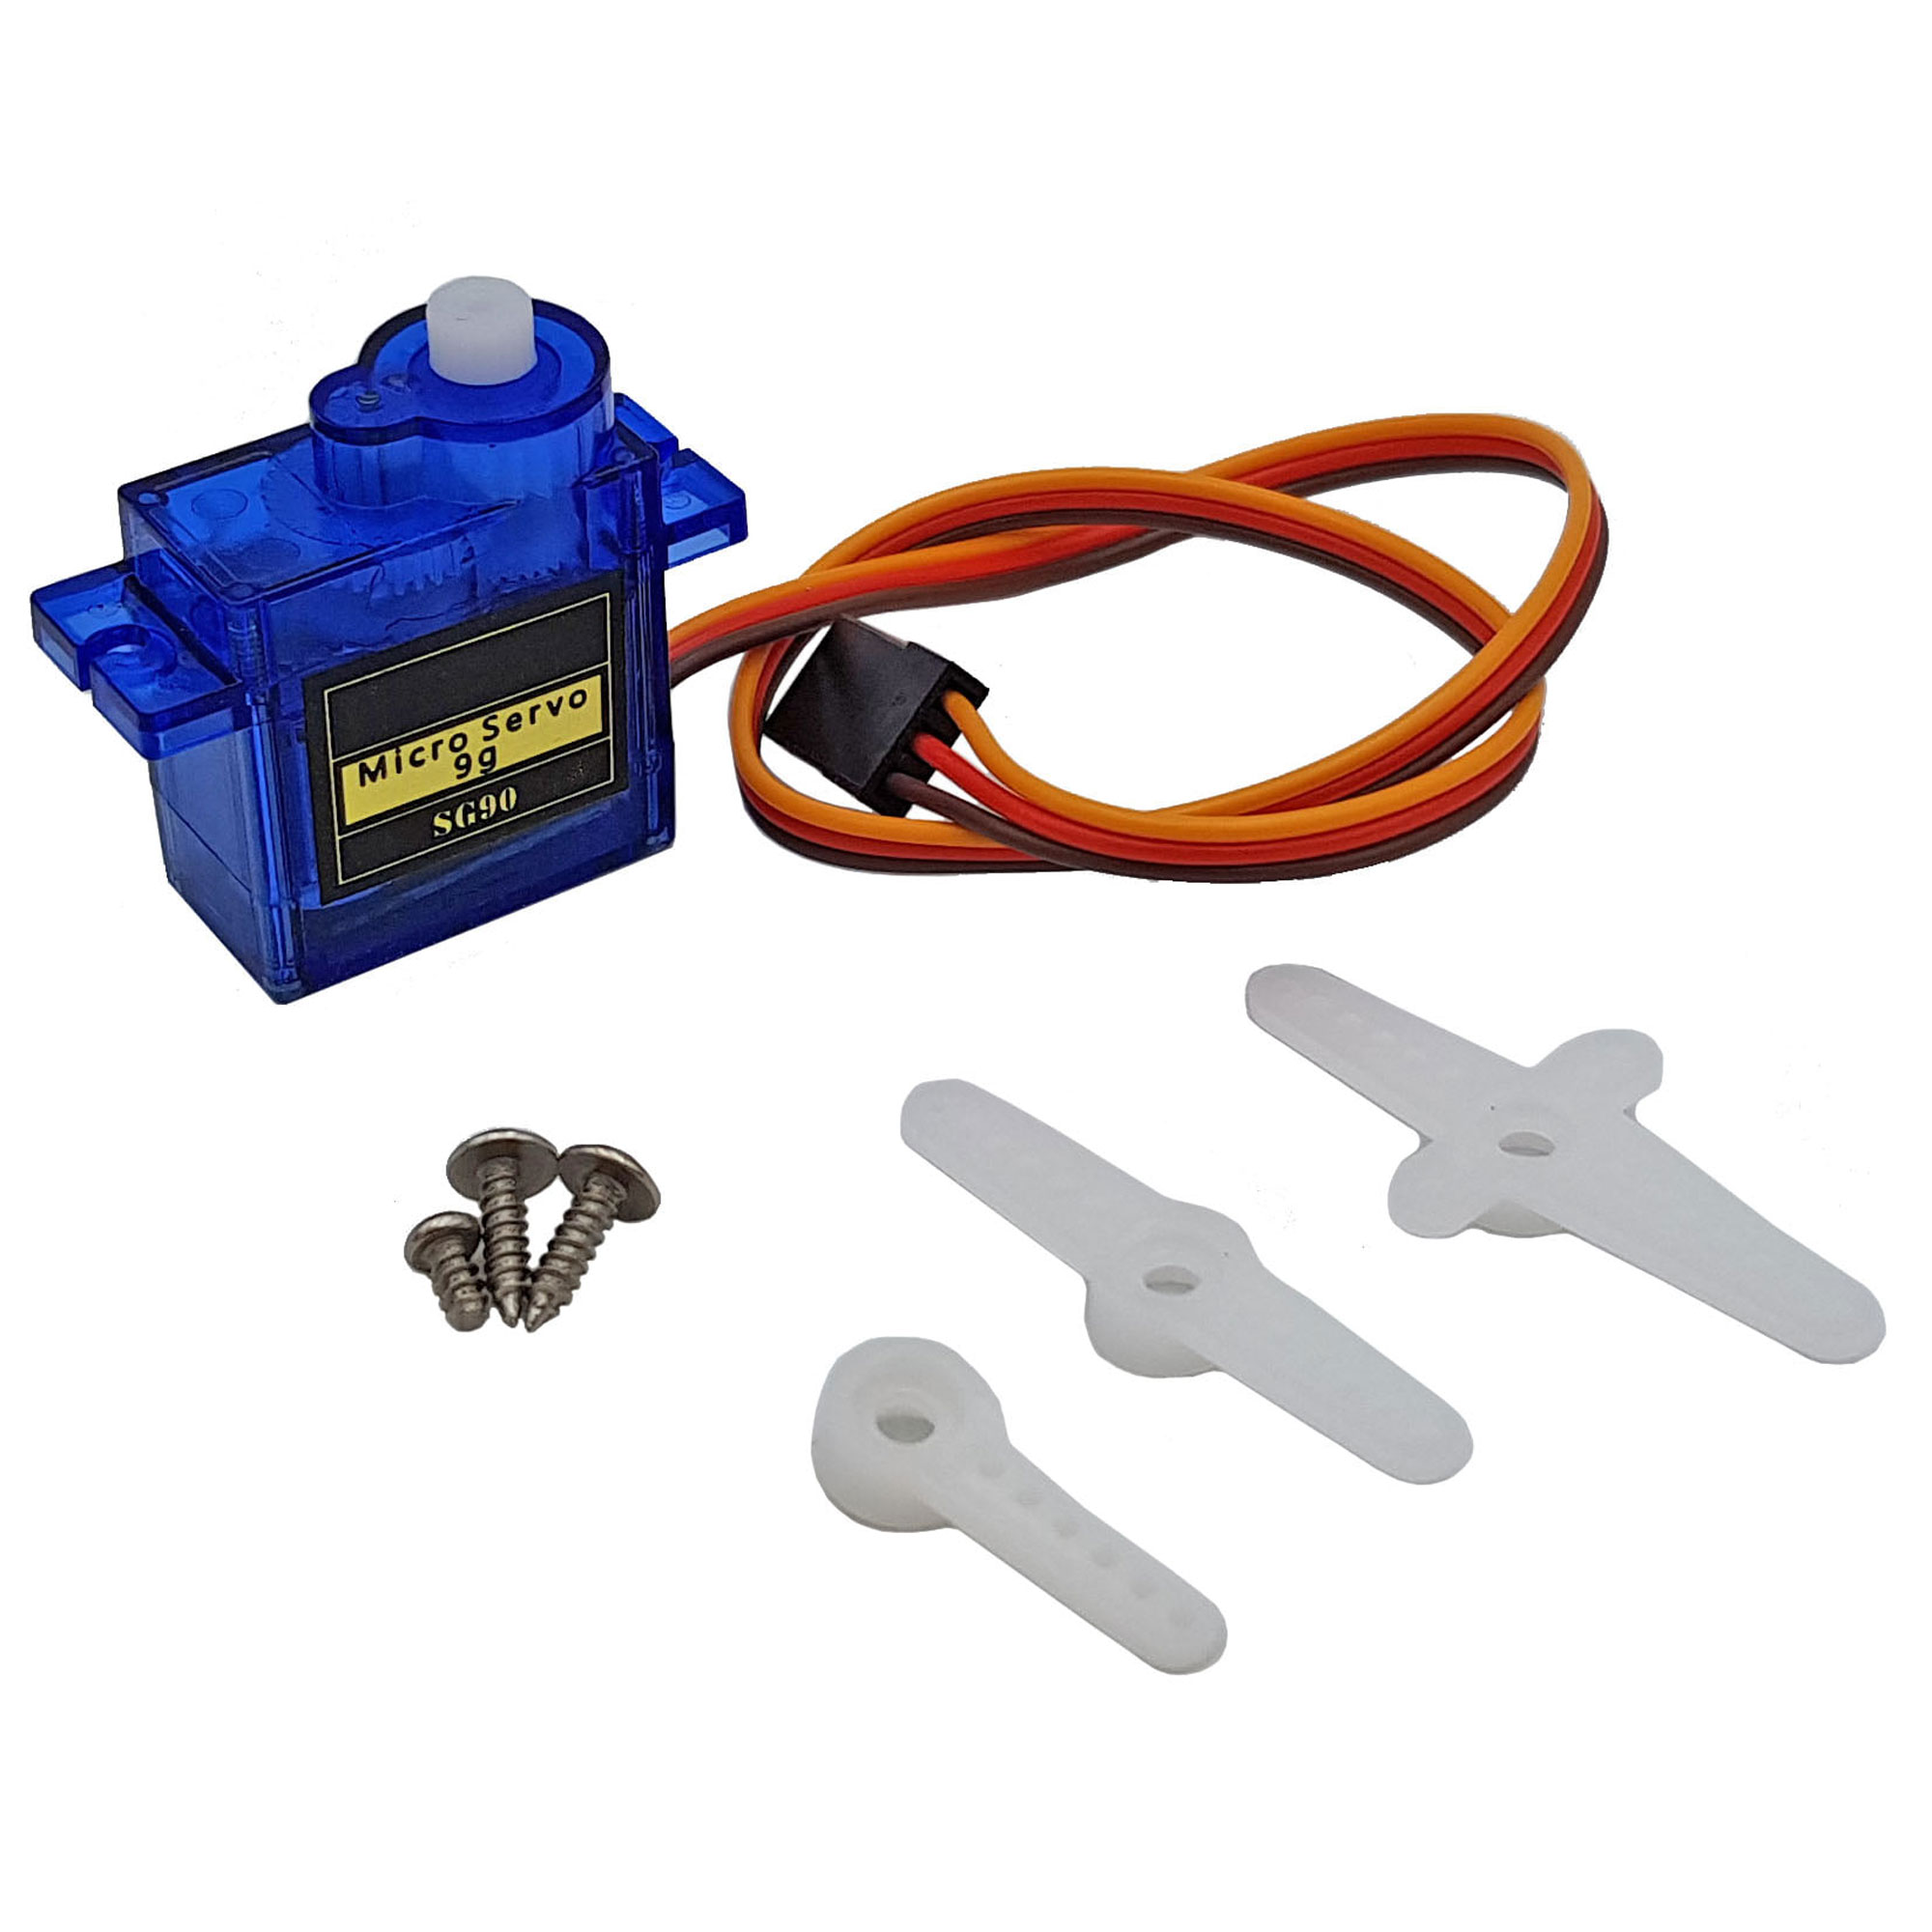
\includegraphics[scale=0.18]{hinh 4.jpg}
    \caption{\textit{Động cơ servo SG90.}}
    \label{fig4}
\end{figure}
\newpage
\begin{itemize}
    \item Hộp Pin 2x18650 Battery Holder có công tắc.\\
    \textbf{Thông số kỹ thuật của hộp Pin}
\end{itemize}
$-$ Sử dụng với Pin 18650 (kích thước: 18 x 65mm).\\
$-$ Tích hợp công tắc dóng ngắt nguồn.\\ 
$-$ Vật liệu: nhựa ABS.\\
$-$ Kích thước: 42 x 22 x 90mm.\\
\begin{figure}[ht!]
    \centering
    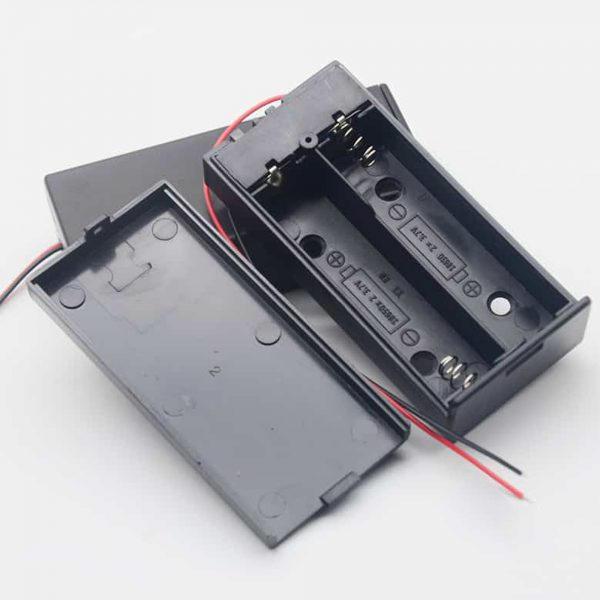
\includegraphics[scale=0.8]{hinh 5.jpg}
    \caption{\textit{Hộp Pin 18650.}}
    \label{fig5}
\end{figure}
\newpage
\begin{itemize}
    \item BreadBoard MB-102.\\
    \textbf{Thông số kỹ thuật BreadBoard MB-102}
\end{itemize}
$-$ Chất liệu: nhựa ABS.\\
$-$ Màu sắc: trắng.\\
$-$ Tổng số lỗ: 830 lỗ (Trong đó 630 lỗ chức năng, 200 lỗ nối nguồn).\\
$-$ Kích thước: 165 x 54 x 8,5mm.\\
$-$ Khối lượng: 77g.\\
\begin{figure}[ht!]
    \centering
    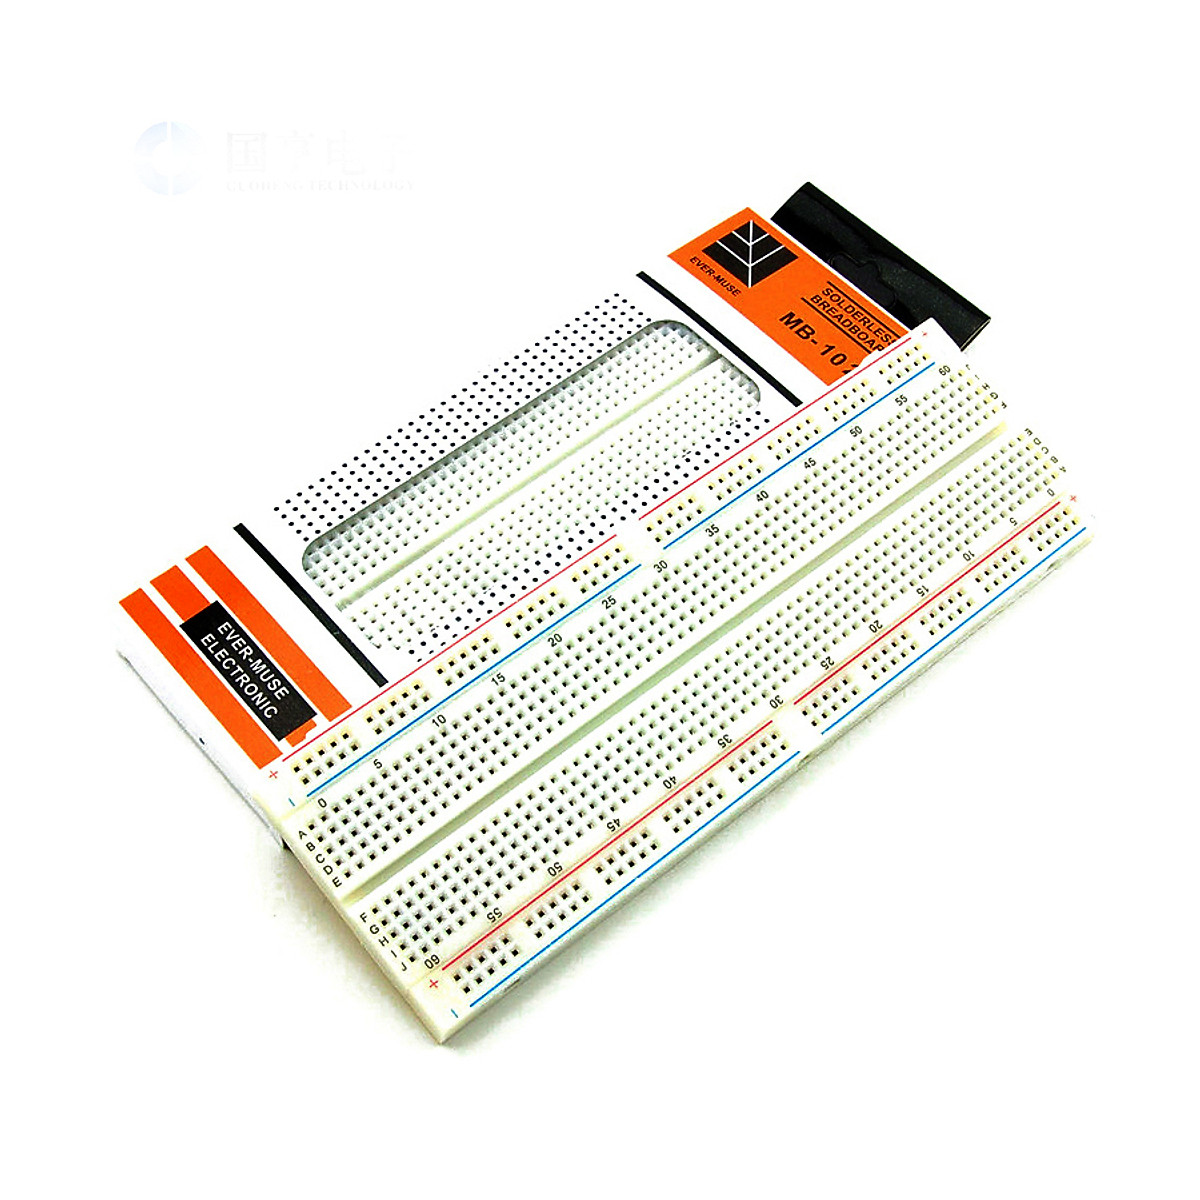
\includegraphics[scale=0.3]{hinh 6.jpg}
    \caption{\textit{BreaBoard MB-102.}}
    \label{fig6}
\end{figure}
\newpage
\subsection{Tiến Hành Nghiên Cứu}
$-$ Lắp ráp các linh kiện.\\
$-$ Sử dụng BreadBoard để test các linh kiện điện tử.\\
$-$ Chạy thử nghiệm hệ thống bên ngoài trước khi lắp đặt.\\
$-$ Cân chỉnh hệ thống và lắp đặt.\\
\subsection{Kết Quả Thực Nghiệm}
$-$ Hoàn thành mô hình thùng rác thông minh, tích hợp các chức năng cho thùng
rác và các chức năng được thực hiện với độ chính xác khá cao.\\
$-$ Hiểu rõ nguyên lý hoạt động, nguyên lý đóng mở, lắp ráp thiết kế thùng rác. Làm tiền đề cho các nghiên cứu tiếp theo.\\
\section{Kết Luận}
\subsection{Kết Quả Đạt Được}
\hspace{0.9cm} Chế tạo thành công và mô hình thùng rác thông minh hoạt động dựa trên các tiêu chí sau: \\
$+$ Tự động mở nắp thùng khi gặp vật cản cách thùng rác 20 cm nhờ vào cảm biến siêu âm (cảm biến khoảng cách).\\
$+$ Nhỏ gọn, tiện dụng giá thành rẻ.\\
$+$ Có thể sử dụng trong các lớp học, văn phòn,...\\
$+$ Thùng rác hoạt động chính xác và tin cậy.\\
\subsection{Hướng Phát Triển Đề Tài}
$+$ Vì đây là mô hình tận thùng rác có sẵn trên thị trường nên độ thẩm mĩ bề ngoài chưa được cao. Nếu có cơ hội được thiết kế về cả ngoại hình lẫn các chi tiết bên trong thì sẽ đẹp hơn.\\
$+$ Thiết kế, chế tạo thùng rác thông minh là đề tài có tính thiết thực trong cuộc sống, với các thay đổi trong thời kì công nghiệp hóa, hiện đại hóa.\\
$+$ Thùng rác thông minh cần được sử dụng rộng rãi vì sự tiện ích của chúng, đồng thời góc phần nâng cao ý thức bảo vệ môi trường của cộng đồng.\\
\newpage
\section{Tài Liệu Tham Khảo}
\begin{thebibliography}{9}
\bibitem{books}
Shamlee Rashinkar - Sneha Ghatole - Swati Kadapatti - Varsha Yadave-
Chaitanya Jambotkar, “\textit{IoT Based Smart Trash Bins–A Step Toward Smart City}”, International Research Journal of Engineering and Technology (IRJET), Dec - 2017.
\bibitem{books}
ThS Nguyễn Đình Phú, “\textit{Giáo Trình Vi Xử Lý}”, NXB Đại Học Quốc Gia 2013.
\bibitem{website}
{https://www.youtube.com/watch?v=zPmKNRAQNmo&t=348s}.
\end{thebibliography}
\end{document}